\section{AWStream: Network Resource Adaptation}

\begin{frame}{Scarce and Variable Bandwidth}

\end{frame}

\begin{frame}{Fidelity vs.\,Freshness}
  \vspace{2em}
  \begin{figure}
    \centering
    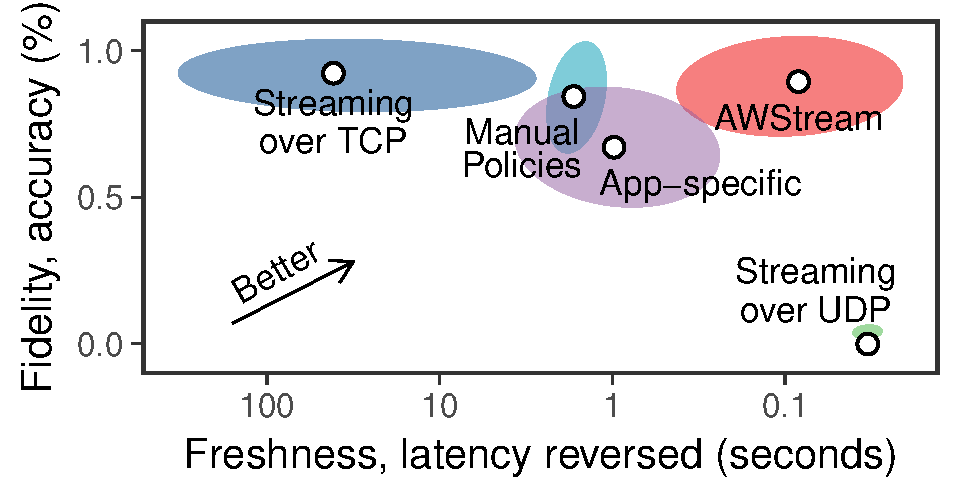
\includegraphics[width=0.8\columnwidth]{figures/fidelity-freshness.pdf}
    \caption{The trade-off space between data freshness and fidelity when facing
      insufficient bandwidth.}
  \end{figure}
\end{frame}

\begin{frame}[t]{Limited Network Resource}
  \vspace{1em}
  \metroset{block=fill}
  \only<2,3>{
    \begin{columns}
      \column{0.5\textwidth}
      \begin{alertblock}{Demand}
        Huge Data Volume at the Edge
      \end{alertblock}
      \column{0.5\textwidth}
      \begin{block}{Resource}
        Insufficient WAN Bandwidth
      \end{block}
    \end{columns}
  }
  \only<4>{
    \begin{columns}
      \column{0.5\textwidth}
      \begin{block}{Demand}
        Huge Data Volume at the Edge
      \end{block}
      \column{0.5\textwidth}
      \begin{alertblock}{Resource}
        Insufficient WAN Bandwidth
      \end{alertblock}
    \end{columns}
  }
  \only<1,5->{
    \begin{columns}

      \column{0.5\textwidth}
      \begin{block}{Demand}
        Huge Data Volume at the Edge
      \end{block}
      \column{0.5\textwidth}
      \begin{block}{Resource}
        Insufficient WAN Bandwidth
      \end{block}
    \end{columns}
  }

  \vspace{1em}

  \only<2>{
    \begin{itemize}
    \item Video surveillance, 3 mbps per camera~\cite{amerasinghe2009h}
    \item Electrical grid monitoring, 1.4 million data points per second~\cite{andersen2016btrdb}
    \item Machine logs, 25 TB daily at Facebook (2009)
    \end{itemize}
  }

  \alt<3>{ \textit{$\ldots$ \alert{Dropcam}, a WiFi video-streaming camera and
      associated cloud backend service for storing and watching the resulting
      video. Dropcam has \alert{the fewest clients} (2,940) $\ldots$. Yet, each
      client uses roughly \alert{2.8 GB} a week and uploads \alert{nearly 19
        times more} than they download, implying that Dropcam users do not often
      watch what they record.}

    Large-scale Measurements of Wireless Network Behavior \\
    \cite{biswas2015large}
  }

  \alt<4>{
    \hypertarget{aws-variation}{}
    \begin{figure}
      \centering
      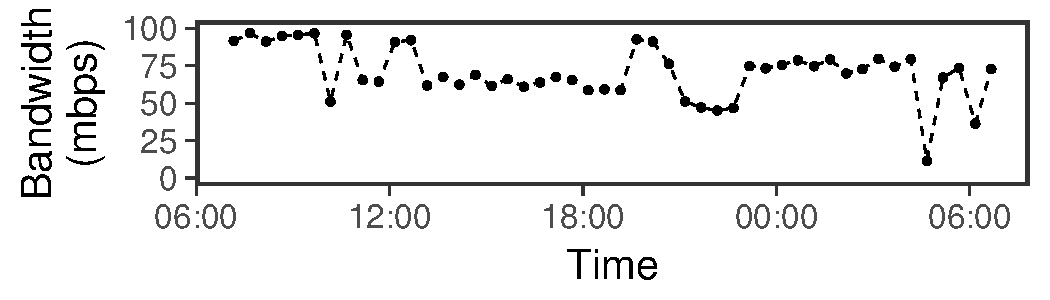
\includegraphics[width=\textwidth]{figures/aws-variation.pdf}
      \caption{Bandwidth variations throughout the day between Amazon EC2
        sites. Similar scarcity and variation for wireless networks, broadband
        access networks and cellular networks
        (\hyperlink{cellular-variation}{backup slides}).}
    \end{figure}
  }

  % \visible<5>{
  %   \begin{figure}
  %     \begin{subfigure}{0.49\textwidth}
  %       \centering
  %       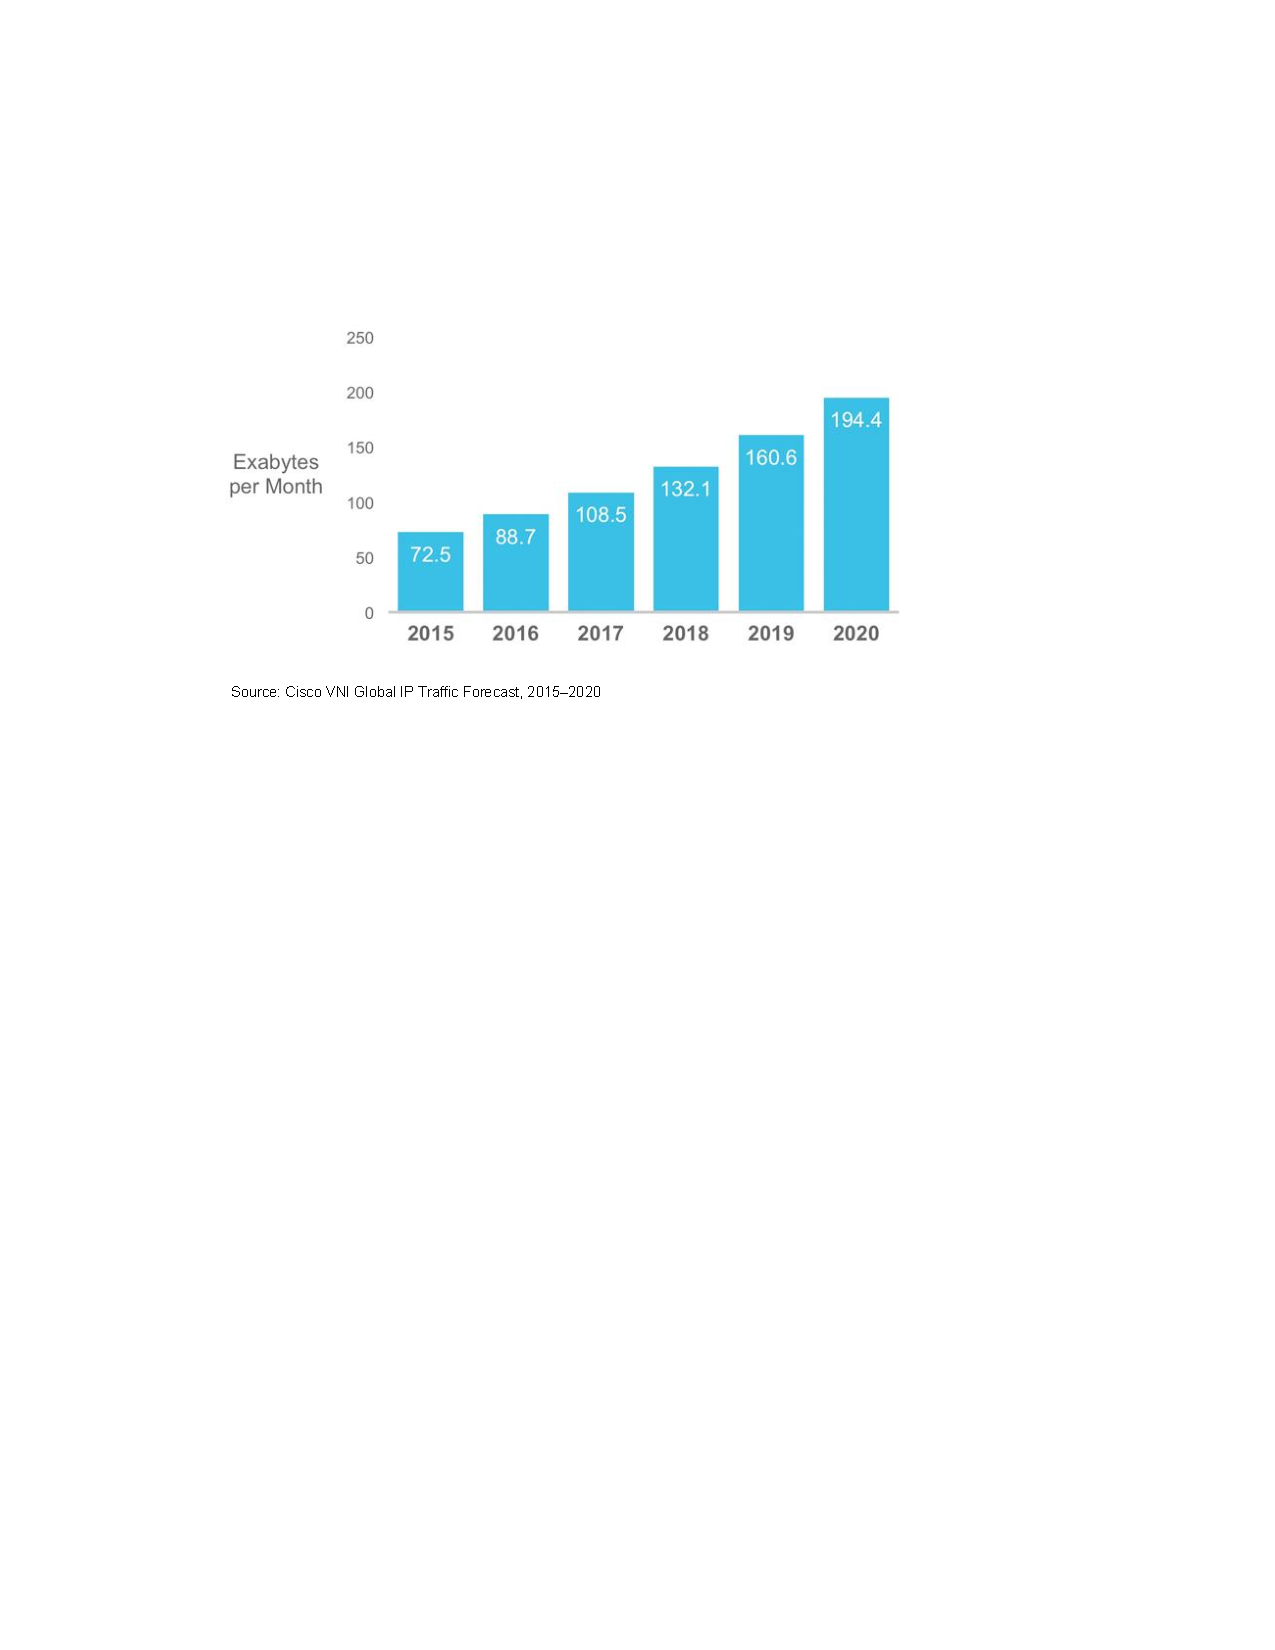
\includegraphics[width=\textwidth]{figures/cisco.pdf}
  %       \caption{Cisco Project Data Growth~\cite{cisco2013zettabyte}}
  %     \end{subfigure}
  %     \hfill
  %     \begin{subfigure}{0.49\textwidth}
  %       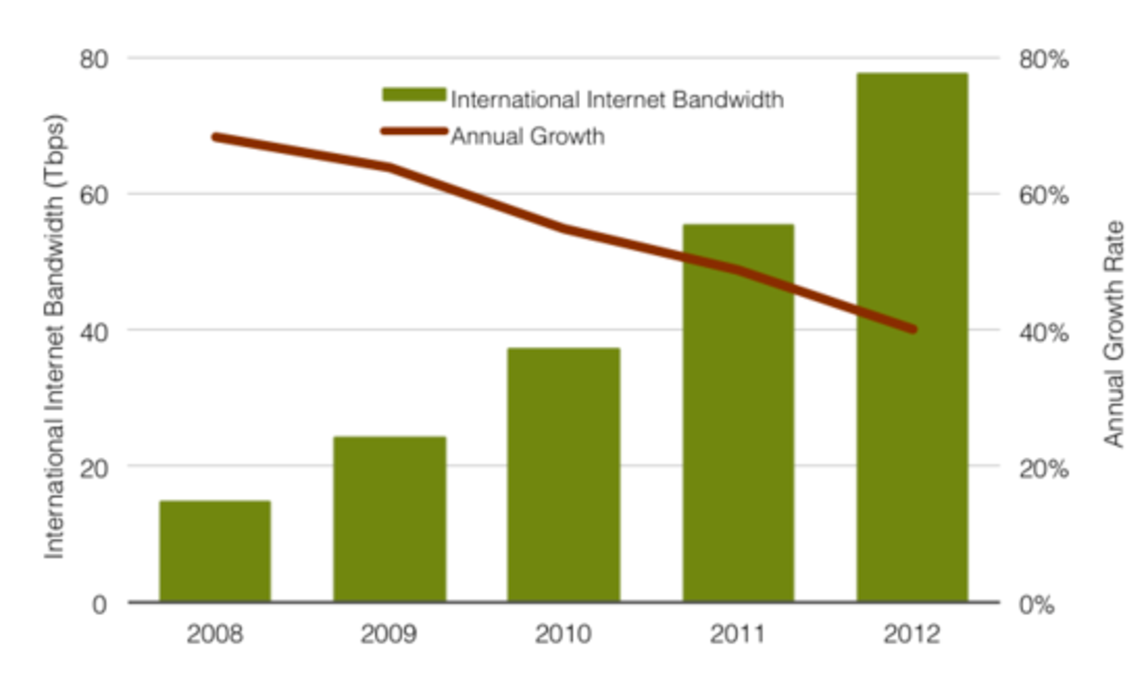
\includegraphics[width=\textwidth]{figures/telegeography.pdf}
  %       \caption{Network backbone capacity growth slows
  %         down~\cite{global2016telegeography}}
  %     \end{subfigure}
  %   \end{figure}
  % }
  \visible<5>{

    What about edge processing? (I will cover in the second half of this talk).

    But communication is not avoidable.

    \begin{itemize}
    \item Large performance gap between the cloud and the edge (GPU/TPU/ASIC).
    \item Aggregation is sometimes necessary in applications.
    \item Last-hop wireless may become the bottleneck.
    \end{itemize}
  }

\end{frame}

\begin{frame}[t]{Fidelity vs.\,Freshness}
  When the network resource is not sufficient:

  \begin{itemize}
  \item TCP ensures data delivery, but hurts latency
  \item UDP sends as fast as possible, uncontrolled packet loss
  \only<2->{
  \item Manual policies (developer heuristics) are sub-optimal
  }
  \only<3>{
      \begin{itemize}
      \item JetStream~\cite{rabkin2014aggregation} uses manual policy
      \item ``if bandwidth is insufficient, switch to sending images at 75\% fidelity,
        then 50\% if still not enough''
      \end{itemize}
    }
  \only<4->{\item Application-specific optimizations don't generalize}
    \only<5>{
      \begin{itemize}
      \item Video streaming often aims at Quality of Experience (limited
        degradation dimension, e.g. maintain 25FPS)
      \item For object detection, resolution matters more than FPS
      \end{itemize}
    }
  \end{itemize}

  \only<7>{
    \begin{figure}
      \centering
      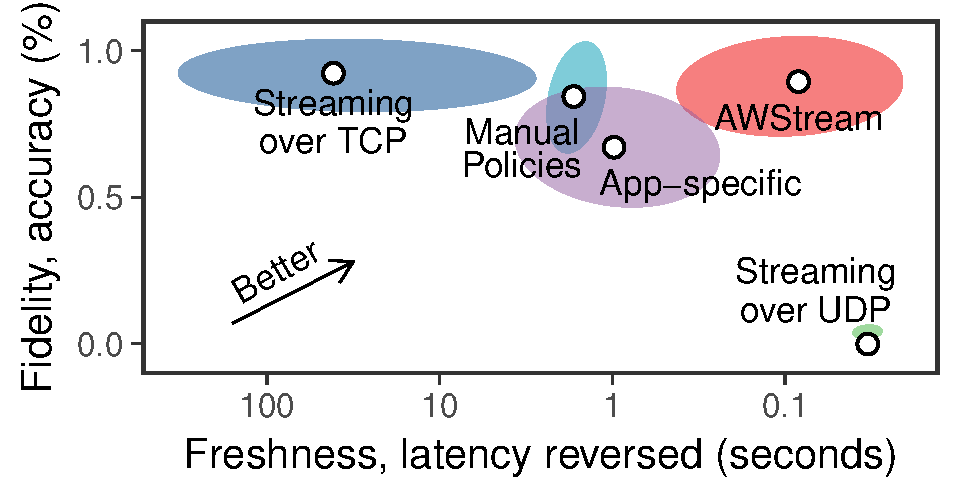
\includegraphics[width=0.8\columnwidth]{figures/fidelity-freshness.pdf}
    \end{figure}
  }
  \only<8>{
    \begin{figure}
      \centering
      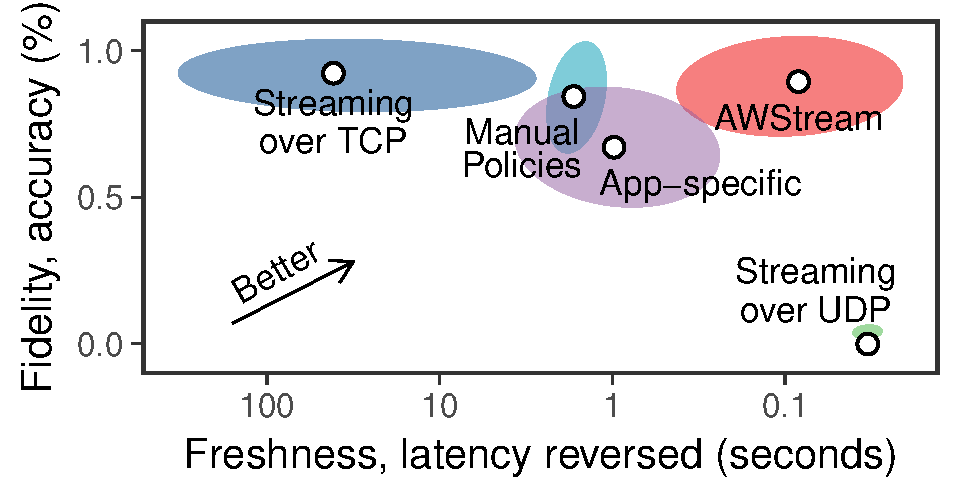
\includegraphics[width=0.8\columnwidth]{figures/fidelity-freshness-full.pdf}
    \end{figure}
  }
\end{frame}

\captionsetup[figure]{labelformat=empty,font=scriptsize,labelfont=scriptsize}
\begin{frame}{Application-specific Optimizations Don't Generalize}
  \pgfplotstableread[row sep=\\,col sep=&]{
    Frame Rate & Bandwidth (normalized) & Accuracy \\
    30 & 100 & 100 \\
    10 & 40 & 92 \\
     5 & 21 & 90 \\
     3 & 13 & 87 \\
     2 & 9 & 84 \\
  }\stationaryframerate
  \pgfplotstableread[row sep=\\,col sep=&]{
    Resolution & Bandwidth (normalized) & Accuracy \\
    1080p & 100 & 100 \\
    900p & 79 & 87 \\
    720p & 54 & 84 \\
    540p & 29 & 71 \\
    360p & 17 & 11 \\
  }\stationaryresolution

  \begin{columns}[t]
    \vspace{1em}
    \column{0.4\textwidth}
    \begin{figure}
      \centering
      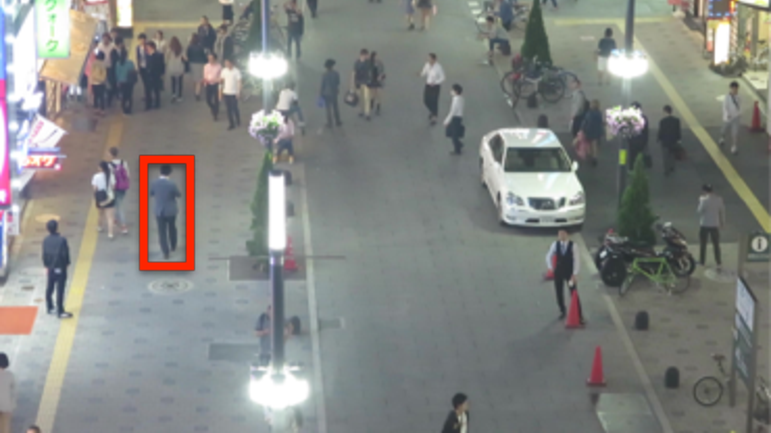
\includegraphics[width=\linewidth]{figures/mot-1.pdf}
      \caption{t=0s, small target in far-field views}
    \end{figure}
    \vspace{-1em}
    \begin{figure}
      \centering
      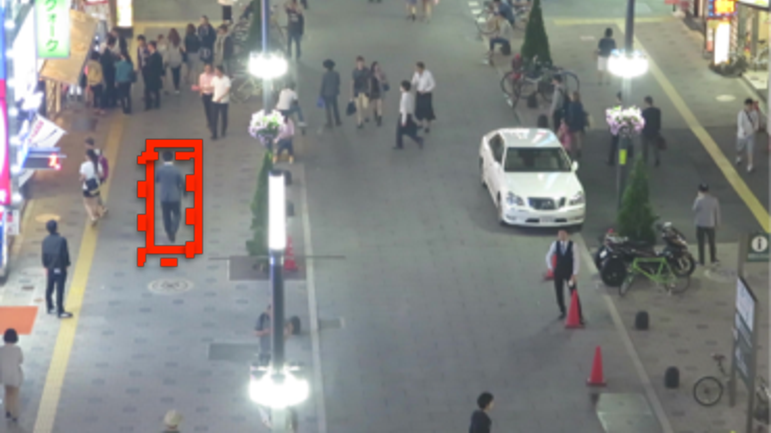
\includegraphics[width=\linewidth]{figures/mot-2.pdf}
      \caption{t=1s, small difference}
    \end{figure}

    \column{0.6\textwidth}

    \only<2>{
      Positive if intersection over union (IOU) larger than 0.5.

      \[
        \text{IOU} = \frac{\text{Area of Intersection}}{\text{Area of Union}}
      \]

      \begin{figure}
        \begin{subfigure}{0.3\textwidth}
          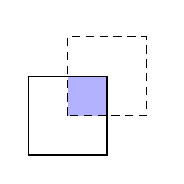
\begin{tikzpicture}
            \fill[color=blue!30] (0.5, 0.5) rectangle (1, 1);
            \node[draw=none] () at (1.5, 1.5) {};
            \draw (0, 0) rectangle (1, 1);
            \draw[densely dashed] (0.5, 0.5) rectangle (1.5, 1.5);
          \end{tikzpicture}
          \caption{IOU=0.14}
        \end{subfigure}
        \begin{subfigure}{0.3\textwidth}
          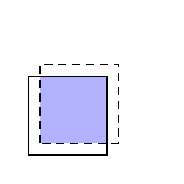
\begin{tikzpicture}
            \fill[color=blue!30] (0.15, 0.15) rectangle (1, 1);
            \node[draw=none] () at (1.5, 1.5) {};
            \draw (0, 0) rectangle (1, 1);
            \draw[densely dashed] (0.15, 0.15) rectangle (1.15, 1.15);
          \end{tikzpicture}
          \caption{IOU=0.57}
        \end{subfigure}
        \begin{subfigure}{0.3\textwidth}
          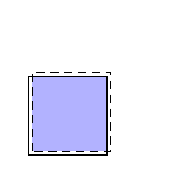
\begin{tikzpicture}
            \fill[color=blue!30] (0.05, 0.05) rectangle (1, 1);
            \node[draw=none] () at (1.5, 1.5) {};
            \draw[densely dashed] (0.05, 0.05) rectangle (1.05, 1.05);
            \draw (0, 0) rectangle (1, 1);
          \end{tikzpicture}
          \caption{IOU=0.82}
        \end{subfigure}
      \end{figure}
    }

    \only<3>{

      F1 score is the harmonic mean of precision and recall, \alert{ranging from
        0 to 1}:

      \begin{table}
        \centering
        \begin{tabular}{| c | c | c |}
          \hline
          & P & N \\
          \hline
          Y & True Positive & False Positive \\
          \hline
          N & False Negative & True Negative \\
          \hline
        \end{tabular}
      \end{table}

      \begin{equation*}
        \begin{split}
          \text{Precision} &= \frac{\text{true positive}}{\text{all positive}} \\
          \text{Recall} &= \frac{\text{true positive}}{\text{all detection}} \\
          \text{F1} &= \frac{2}{\frac{1}{\text{Recall}} + \frac{1}{\text{Precision}}}
        \end{split}
      \end{equation*}

    }
    \only<4->{
      \begin{tikzpicture}
        \tikzstyle{every node}=[font=\footnotesize]
        \begin{axis}[
          ybar,
          bar width               = .4cm,
          width                   = 1.1\textwidth,
          height                  = 0.4\textheight,
          legend style            = {at = {(0.5, 1.4)}, anchor = north,legend columns = -1},
          symbolic x coords       = {30, 10, 5, 3, 2},
          xtick                   = data,
          enlarge x limits        = 0.15,
          ymin                    = 0,
          ymax                    = 130,
          xlabel                  = {Frame Rate},
          nodes near coords,
          nodes near coords align = {vertical},
          ]
          \addplot+[visible on=<6->] table[x=Frame Rate,y=Bandwidth (normalized)]{\stationaryframerate};
          \addplot+[visible on=<5->] table[x=Frame Rate,y=Accuracy]{\stationaryframerate};
          \legend{Bandwidth (normalized), Accuracy}
        \end{axis}
      \end{tikzpicture}

      \vspace{1em}

      \visible<7>{
        \begin{tikzpicture}
          \tikzstyle{every node}=[font=\footnotesize]
          \begin{axis}[
            ybar,
            bar width               = .4cm,
            width                   = 1.1\textwidth,
            height                  = 0.4\textheight,
            symbolic x coords       = {1080p, 900p, 720p, 540p, 360p},
            xtick                   = data,
            enlarge x limits        = 0.15,
            nodes near coords,
            nodes near coords align = {vertical},
            ymin                    = 0,
            ymax                    = 130,
            xlabel                  = {Resolution},
            ]
            \addplot table[x = Resolution, y = Bandwidth (normalized)]{\stationaryresolution};
            \addplot table[x = Resolution, y = Accuracy]{\stationaryresolution};
            \legend{}
          \end{axis}
        \end{tikzpicture}
      }
    }
  \end{columns}
\end{frame}


\begin{frame}{Application-specific Optimizations Don't Generalize}
  \captionsetup[figure]{labelformat=empty,font=scriptsize,labelfont=scriptsize}

  \pgfplotstableread[row sep=\\,col sep=&]{
    Frame Rate & Bandwidth (normalized) & Accuracy \\
    30 & 100 & 100 \\
    10 & 65 & 64 \\
    5 & 46 & 32 \\
    3 & 34 & 18 \\
    2 & 27 & 10 \\
  }\mobileframerate
  \pgfplotstableread[row sep=\\,col sep=&]{
    Resolution & Bandwidth (normalized) & Accuracy \\
    1080p & 100 & 100 \\
    900p & 69 & 99 \\
    720p & 49 & 97 \\
    540p & 33 & 93 \\
    360p & 22 & 87 \\
  }\mobileresolution

  \begin{columns}[t]
    \column{0.4\textwidth}
    \vspace{2em}
    \begin{figure}
      \centering
      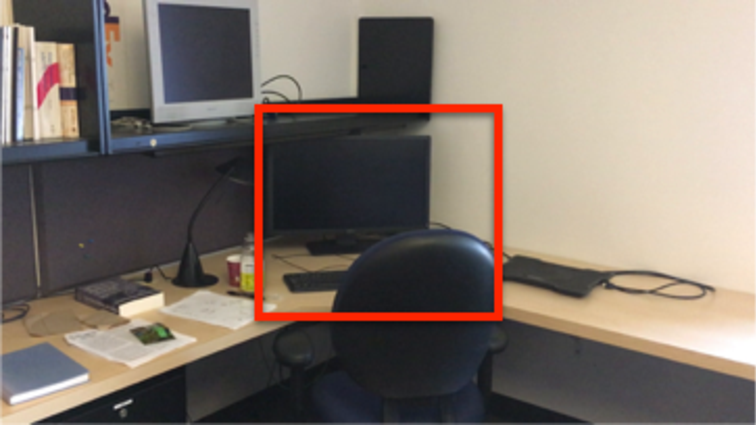
\includegraphics[width=\linewidth]{figures/darknet-1.pdf}
      \caption{t=0s, nearby and large targets}
    \end{figure}
    \vspace{-1em}
    \begin{figure}
      \centering
      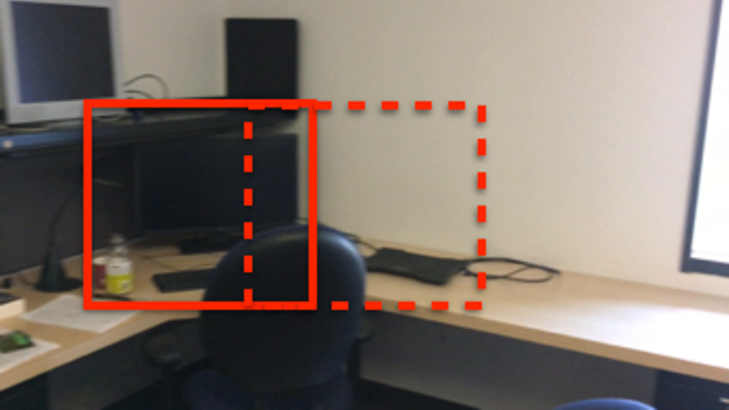
\includegraphics[width=\linewidth]{figures/darknet-2.pdf}
      \caption{t=1s, large difference}
    \end{figure}

    \column{0.6\textwidth}
    \vspace{1.5em}

    \begin{tikzpicture}
      \tikzstyle{every node}=[font=\footnotesize]
      \begin{axis}[
        ybar,
        bar width               = .4cm,
        width                   = 1.1\textwidth,
        height                  = 0.4\textheight,
        legend style            = {at = {(0.5, 1.4)}, anchor = north,legend columns = -1},
        symbolic x coords       = {30, 10, 5, 3, 2},
        xtick                   = data,
        enlarge x limits        = 0.15,
        ymin                    = 0,
        ymax                    = 130,
        xlabel                  = {Frame Rate},
        nodes near coords,
        nodes near coords align = {vertical},
        ]
        \addplot table[x=Frame Rate,y=Bandwidth (normalized)]{\mobileframerate};
        \addplot table[x=Frame Rate,y=Accuracy]{\mobileframerate};
        \legend{Bandwidth (normalized), Accuracy}
      \end{axis}
    \end{tikzpicture}

    \vspace{1em}

    \begin{tikzpicture}
      \tikzstyle{every node}=[font=\footnotesize]
      \begin{axis}[
        ybar,
        bar width               = .4cm,
        width                   = 1.1\textwidth,
        height                  = 0.4\textheight,
        symbolic x coords       = {1080p, 900p, 720p, 540p, 360p},
        xtick                   = data,
        enlarge x limits        = 0.15,
        nodes near coords,
        nodes near coords align = {vertical},
        ymin                    = 0,
        ymax                    = 130,
        xlabel                  = {Resolution},
        ]
        \addplot table[x = Resolution, y = Bandwidth (normalized)]{\mobileresolution};
        \addplot table[x = Resolution, y = Accuracy]{\mobileresolution};
        \legend{}
      \end{axis}
    \end{tikzpicture}
  \end{columns}
\end{frame}

\begin{frame}[t]{Making Adaptation Practical is Challenging}
  \vspace{1em}

  \metroset{block=fill}

  \begin{block}{Goal}
    Minimize bandwidth while maximizing application accuracy
  \end{block}

  \only<2-7>{
    \textbf{Challenges}:

    \begin{enumerate}
      \visible<2->{\item Application-specific optimizations don't generalize.}
      \visible<5->{
        \begin{itemize}
        \item APIs: \texttt{maybe} operators to express adaptation.
        \end{itemize}
      }
      \visible<3->{
      \item It requires expertise and manual work to explore multidimensional adaptation.
      }
      \visible<6->{
        \begin{itemize}
        \item Profiling: automatically learn Pareto-optimal strategy with
          multi-dimensional exploration.
        \end{itemize}
      }
      \visible<4->{
      \item The adaptation happens at the runtime.
      }
      \visible<7->{
        \begin{itemize}
        \item Engineering an adaptation system to balance latency and accuracy.
        \end{itemize}
      }
    \end{enumerate}
  }
  \only<8>{
    \begin{figure}
      \centering
      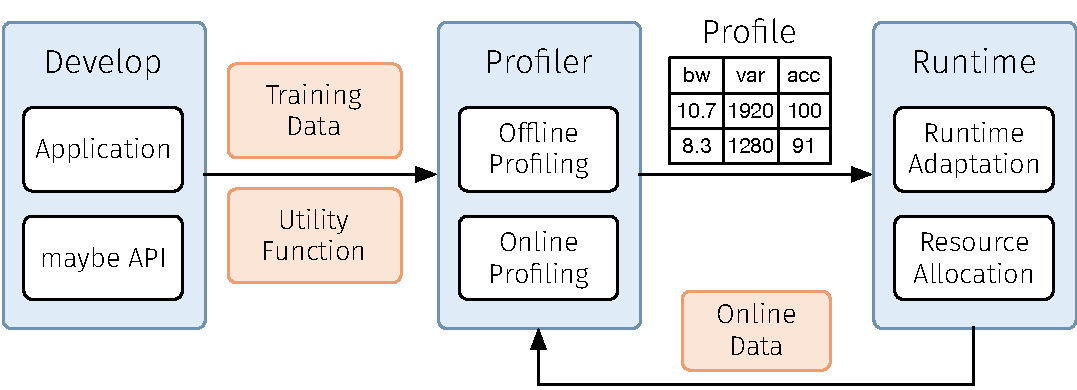
\includegraphics[width=0.8\linewidth]{figures/arch.pdf}
    \end{figure}
  }
\end{frame}

% \begin{frame}{System Architecture Overview}
%   \centering
%   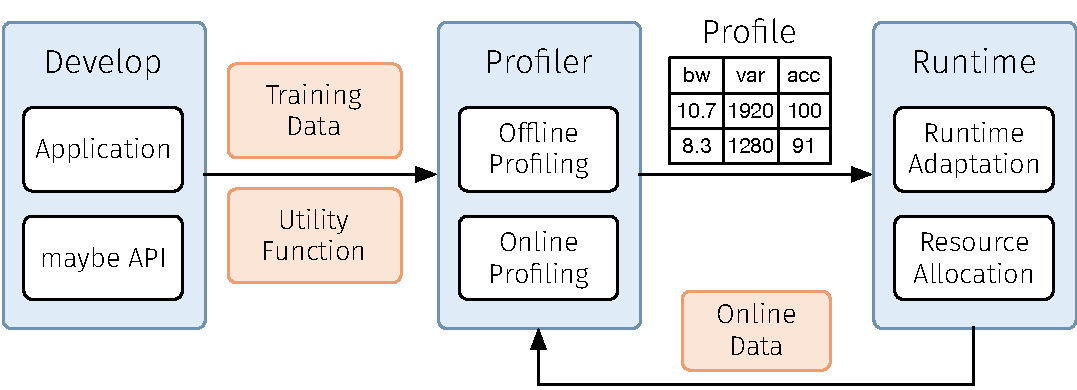
\includegraphics[width=0.8\linewidth]{figures/arch.pdf}\\
%   \begin{tikzpicture}
%     \draw[dashed] (0,0) -- (10,0);
%   \end{tikzpicture}
%   \centering
%   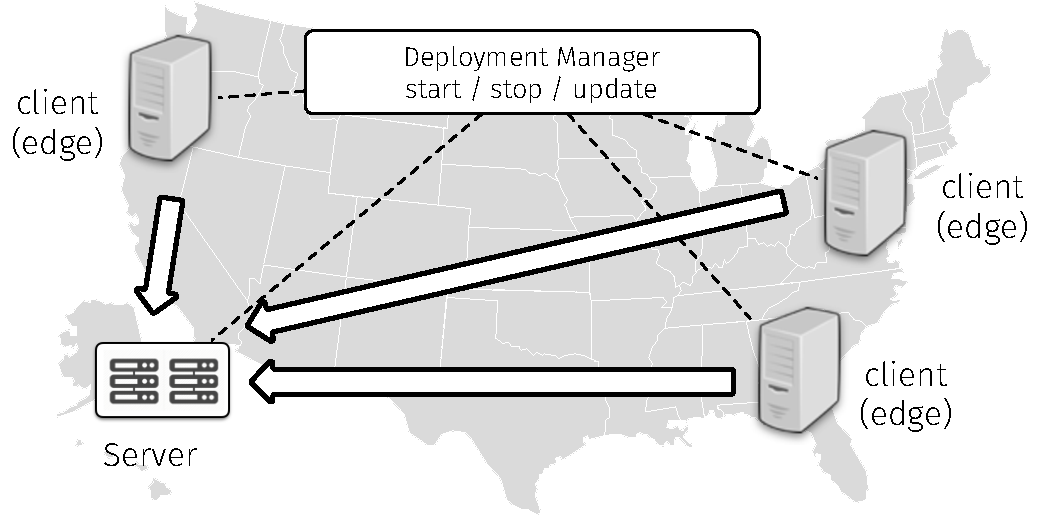
\includegraphics[width=0.7\linewidth]{figures/arch-2.pdf}
% \end{frame}

%%% Local Variables:
%%% mode: latex
%%% TeX-master: "../talk"
%%% TeX-engine: xetex
%%% End:


\begin{frame}{Making Adaptation Practical is Challenging}

  \textbf{Goal}: Minimize bandwidth while maximizing application accuracy

  \begin{block}{My block}
    Content of my block.
  \end{block}

  \textbf{Challenges}:
  \begin{itemize}
  \item Application-specific optimizations don't generalize
  \item API. \texttt{maybe} operators to express adaptation.
  \item It requires expertise and manual work to explore multidimensional
    adaptation
  \item Profiling: automatically learn Pareto-optimal strategy with
    multi-dimensional exploration.
  \item The adaptation needs to happen at the runtime: no viable system yet
  \item runtime adaptation balances the latency with data accuracy
  \end{itemize}
\end{frame}

\begin{frame}{System Architecture Overview}
  \centering
  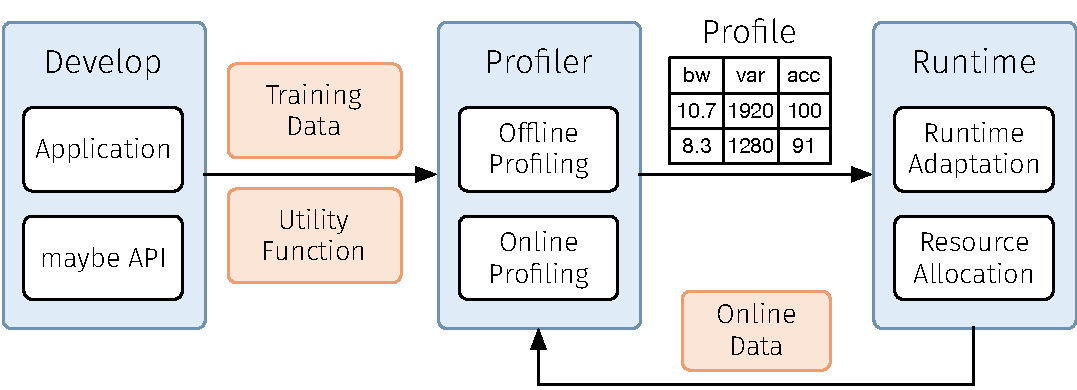
\includegraphics[width=0.8\linewidth]{figures/arch.pdf}\\
  \begin{tikzpicture}
    \draw[dashed] (0,0) -- (10,0);
  \end{tikzpicture}
  \centering
  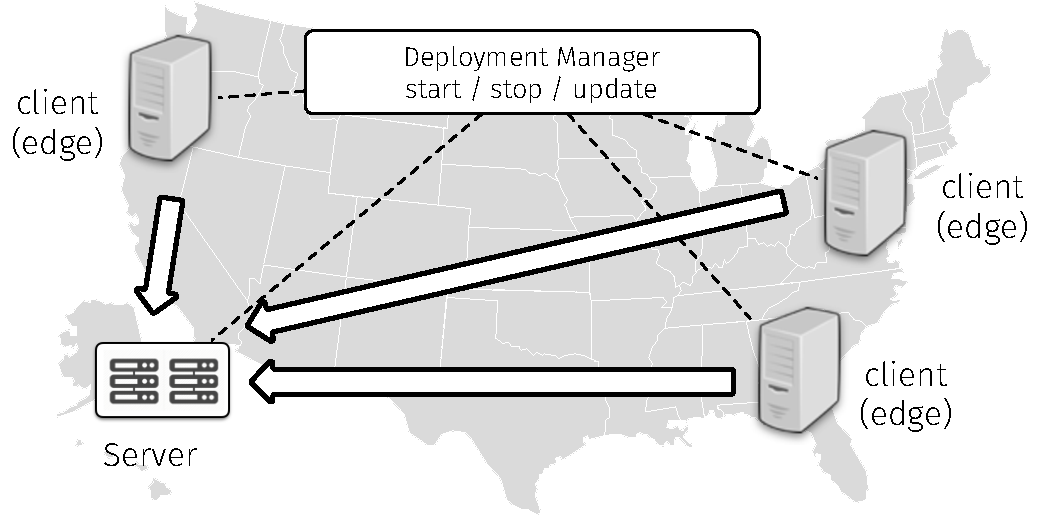
\includegraphics[width=0.7\linewidth]{figures/arch-2.pdf}
\end{frame}

\begin{frame}{(1) Stream Processing APIs}
  \vspace{1em}
  \centering
  \begin{tikzpicture}
    \node[bn, minimum width=2cm] (op) {Operator};
    \node [left=1cm of op] (left) {Data Stream};
    \node [right=1cm of op] (right) {Data Stream};
    \draw[to] (left) -- (op);
    \draw[to] (op) -- (right);
  \end{tikzpicture}

  \visible<2->{
    \vspace{1em}
    \scalebox{0.7}{
      \begin{tikzpicture}
        \node[bn, minimum width=3cm] (op) {map(f)};
        \node [left=1cm of op] (left) {$\{x_1, x_2, x_3, x_4, \ldots \}$};
        \node [right=1cm of op] (right) {$\{f(x_1), f(x_2), f(x_3), f(x_4), ...\}$};
        \draw[to] (left) -- (op);
        \draw[to] (op) -- (right);

        \node[bn, minimum width=3cm, below=0.5cm of op] (op2) {window(2, f)};
        \node [left=1cm of op2] (left2) {$\{x_1, x_2, x_3, x_4, \ldots \}$};
        \node [right=1cm of op2] (right2) {$\{f(x_1, x_2), f(x_3, x_4), ...\}$};
        \draw[to] (left2) -- (op2);
        \draw[to] (op2) -- (right2);

        \visible<4->{
        \node[bn, minimum width=3cm, below=0.5 of op2] (op3) {maybe($\vec{k}$, f)};
        \node [left=1cm of op3] (left3) {$\{x_1, x_2, x_3, x_4, \ldots \}$};
        \node [right=1cm of op3] (right3) {$\{f(x_1, k_{i_1}), f(x_2, k_{i_2}), f(x_3, k_{i_3}),
          f(x_4, k_{i_4}), ...\}$};
        \draw[to] (left3) -- (op3);
        \draw[to] (op3) -- (right3);
        }
      \end{tikzpicture}
    }
  }
  
  \visible<3->{
  \begin{table}
    \scriptsize
    \begin{tabular}{ c r l }
      \toprule
      \multirow{4}{*}{Normal}
      & \textit{map} (f: I $\Rightarrow$ O) & Stream<I> $\Rightarrow$ Stream<O> \\
      & \textit{skip} (i: Integer) & Stream<I> $\Rightarrow$
                                     Stream<I> \\
      & \textit{window} (count: Integer, f: Vec<I> $\Rightarrow$ O) & Stream<I> $\Rightarrow$
                                                                      Stream<O> \\
      & ... & ... \\
      \midrule \visible<5->{
      \multirow{4}{*}{Adaptation}
      & \textit{maybe} (knobs: Vec<T>, f:  (T, I) $\Rightarrow$ I) & Stream<I> $\Rightarrow$
                                                                     Stream<I> \\
      & \textit{maybe\_skip} (knobs: Vec<Integer>) & Stream<I> $\Rightarrow$ Stream<I> \\
      & \textit{maybe\_head} (knobs: Vec<Integer>) & Stream<Vec<I>{}> $\Rightarrow$
                                                     Stream<Vec<I>{}> \\
      & ... & ... \\
      \bottomrule
      }
    \end{tabular}
  \end{table}
  }
\end{frame}

\begin{frame}[fragile]{\texttt{maybe(knobs: Vec<T>, f: (T, I) => I)}}
  \begin{tikzpicture}[
    level distance=2cm,
    level 1/.style={sibling distance=4cm},
    edge from parent/.style={->,draw},
    >=latex]
    \node[bn] {
\begin{lstlisting}
let quantized_stream = vec![1, 2, 3, 4].into_stream()
    .maybe(vec![2, 4], |k, val| val / k)
    .collect();
\end{lstlisting}
    }
    child {node[yn] (c1) {[1, 2, 3, 4]} edge from parent node [left] {no degradation}}
    child {node[yn] (c2) {[0, 1, 1, 2]} edge from parent node [left] {k = 2}}
    child {node[yn] (c3) {[0, 0, 0, 1]} edge from parent node [left] {k = 4}};
  \end{tikzpicture}

  \pause
  \vspace{2em}
  We rewrite the video streaming application as follows{\let\thefootnote\relax\footnote{{Example code in
    Rust, simplified for presentation.}}},

  \centering
  \begin{lstlisting}
let app = Camera::new((1920, 1080), 30)
    .maybe_downsample(vec![(1600, 900), (1280, 720)])
    .maybe_skip(vec![2, 5])
    .map(|frame| pedestrian_detect(frame))
    .compose();
  \end{lstlisting}
\end{frame}

%%% Local Variables:
%%% mode: latex
%%% TeX-master: "../talk"
%%% TeX-engine: xetex
%%% End:

\begin{frame}[fragile]{(2) Profiling}
  \vspace{1em}
  \centering
  \begin{tikzpicture}
    \node[draw=none] (center) {};
    \node[bn, above=1cm of center] (code) {
\begin{lstlisting}
let app = Camera::new((1920, 1080), 30)
    .maybe_downsample(vec![(1600, 900), (1280, 720)])
    .maybe_skip(vec![2, 5])
    .map(|frame| pedestrian_detect(frame))
    .compose();
\end{lstlisting}
    };
    
    \visible<2->{
      \node[bn, minimum width=3.5cm, left=2cm of center] (data) {Training Data};
    }
    \visible<3->{
      \node[bn, minimum width=3.5cm, right=2cm of center] (func) {Accuracy
        Function};
    }
    
    \visible<4->{
      \node[draw=none, below=1cm of center] (target) {};
      \node[draw=none, left=0.2cm of target] (targeta) {};
      \node[draw=none, right=0.2cm of target] (targetb) {};
      \draw[to] (code) -- (target);
      \draw[to] (data) -- (targeta);
      \draw[to] (func) -- (targetb);
    }
  \end{tikzpicture}

  \visible<4->{
  \vspace{-1em}
  \footnotesize
  \begin{table}
    \begin{tabular}{c c c c}
      \toprule
      downsample & skip & bandwidth & accuracy \\
      \midrule
      (1920, 1080) & 0 & 10.7 & 1.0 \\
      (1600, 900)  & 0 & 8.3 & 0.88  \\
      (1280, 720)  & 0 & 6.3 & 0.87 \\
      (1920, 1080) & 2 & 9.3 & 0.90 \\
      ... & ... & ... & ... \\
      \bottomrule
    \end{tabular}
  \end{table}
  }
\end{frame}

\begin{frame}{Profile: Pareto-optimal Strategy}
  \begin{columns}
    \begin{column}{0.39\textwidth}
      \centering
      \only<1->{
      \begin{tikzpicture}
        \begin{axis}[
          width  = \textwidth,
          xlabel = Bandwidth (normalize),
          ylabel = Accuracy,
          ymin   = 0,
          ymax   = 1,
          ytick  = {0, 1},
          xmin   = 0,
          xmax   = 1,
          xtick  = {0, 1},
          ]

          \only<2->{
            \addplot[color=red, mark=x, only marks] coordinates {(0.95,0.95)};
          }
          \only<3->{
            \addplot[color=red, mark=x, only marks] coordinates {(0.90,0.92)};
          }
          \only<4->{
            \addplot[color=red, mark=x, only marks] coordinates {(0.85,0.90)};
          }
          \only<5->{
            \addplot[color=red, mark=x, only marks] coordinates {(0.70,0.80)};
          }
          \only<6->{
            \addplot[color=blue, mark=x, only marks] coordinates {(0.75,0.75)};
          }
          \only<7->{
            \addplot[color=red, mark=x, only marks] coordinates {
              (0.6, 0.7)
              (0.5, 0.65)
              (0.4, 0.55)
              (0.3, 0.50)
              (0.2, 0.45)
              (0.1, 0.20)
            };
            \addplot[color=blue, mark=x, only marks] coordinates {
              (0.83, 0.62)
              (0.80, 0.59)
              (0.74, 0.60)
              (0.63, 0.56)
              (0.61, 0.36)
              (0.51, 0.34)
              (0.50, 0.40)
              (0.49, 0.41)
              (0.47, 0.42)
              (0.46, 0.30)
              (0.44, 0.25)
              (0.24, 0.20)
              (0.10, 0.10)
            };
          }
          
        \end{axis}
      \end{tikzpicture}
      }
    \end{column}

    \begin{column}{0.59\linewidth}
      \scriptsize
      \begin{table}
        \centering
        \begin{tabular}{r l}
          \toprule
          \textbf{Symbol} & \textbf{Description} \\
          \midrule
          $n$ & number of degradation operations \\
          $k_i$ & the \textit{i}-th degradation knob \\
          $c = [k_{1}, k_{2}, ... k_{n}]$ & one specific configuration \\
          $\mathbb{C}$ & the set of all configurations \\
          \midrule
          $B(c)$ & bandwidth requirement for $c$ \\
          $A(c)$ & accuracy measure for $c$ \\
          $\mathbb{P}$ & Pareto-optimal set \\
          \bottomrule
        \end{tabular}
      \end{table}

      \visible<8->{
        \[
          \mathbb{P} = \{ c \in \mathbb{C} :
          \underbrace{\{ c' \in \mathbb{C}: B(c') < B(c),
            A(c') > A(c) \}}_{\text{set of better configurations $c'$}}
          = \varnothing\}
        \]

        See red markers in the figure.
      }
        
    \end{column}
  \end{columns}
\end{frame}

%%% Local Variables:
%%% mode: latex
%%% TeX-master: "../talk"
%%% TeX-engine: xetex
%%% End:


\begin{frame}{(3) Runtime Adaptation}
  \begin{figure}
    \centering
    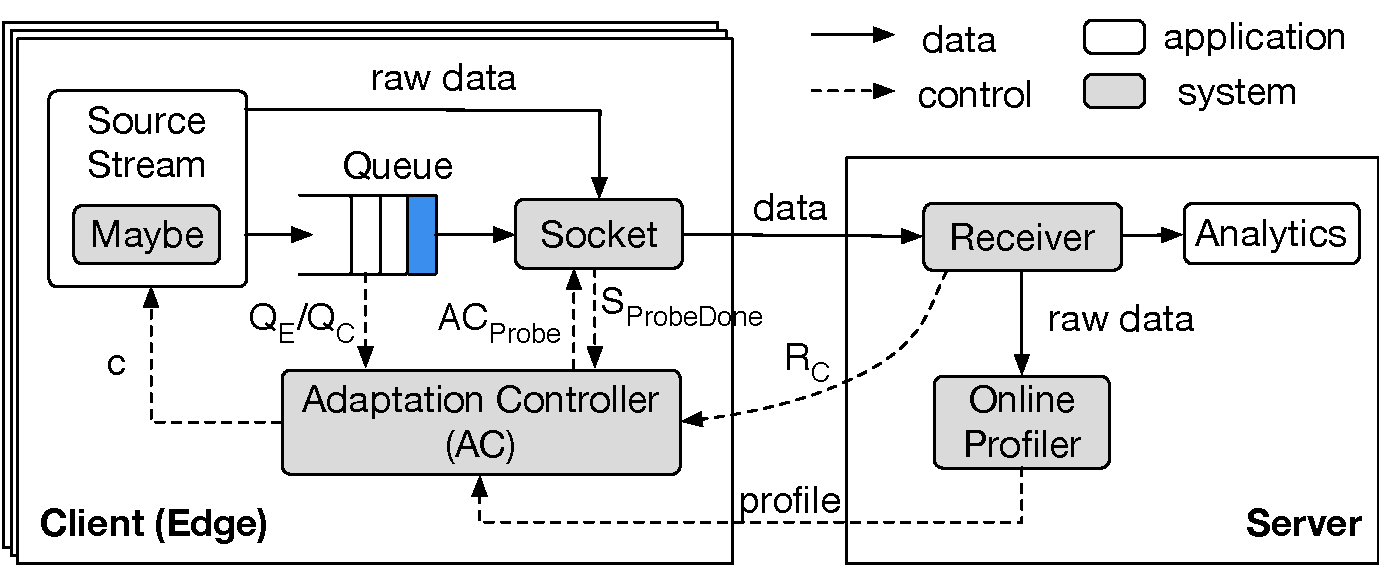
\includegraphics[width=\linewidth]{figures/runtime-adaptation.pdf}
  \end{figure}
\end{frame}

\begin{frame}{Applications}
  \begin{table}
    \scriptsize
    \centering
    \begin{tabular}{c c c c}
      \toprule
      Application & Knobs & Accuracy & Dataset \\
      \midrule
      \specialcell{Augmented\\Reality}
                  & \specialcell{resolution \\ frame rate \\ quantization }
                  & \specialcell{F1 score\\\cite{Rijsbergen:1979:IR:539927}}
                  & \specialcell{iPhone video clips\\training: office (24s)\\testing: home (246s)} \\
      
      \midrule
      \specialcell{Pedestrian\\Detection}
                  & \specialcell{resolution \\ frame rate \\ quantization }
                  & F1 score
                          & \specialcell{MOT16~\cite{milan2016mot16}\\training: MOT16-04\\testing: MOT16-03} \\
      \midrule
      \specialcell{Log Analysis\\(Top-K, K=50)}
                  & \specialcell{head (N) \\ threshold (T) }
                  & \specialcell{Kendall's $\tau$\\\cite{abdi2007kendall}}
                  & \specialcell{\href{https://www.sec.gov}{SEC.gov} logs~\cite{edgarlog} \\ training: 4 days \\
      testing: 16 days} \\
      \bottomrule
    \end{tabular}
  \end{table}

  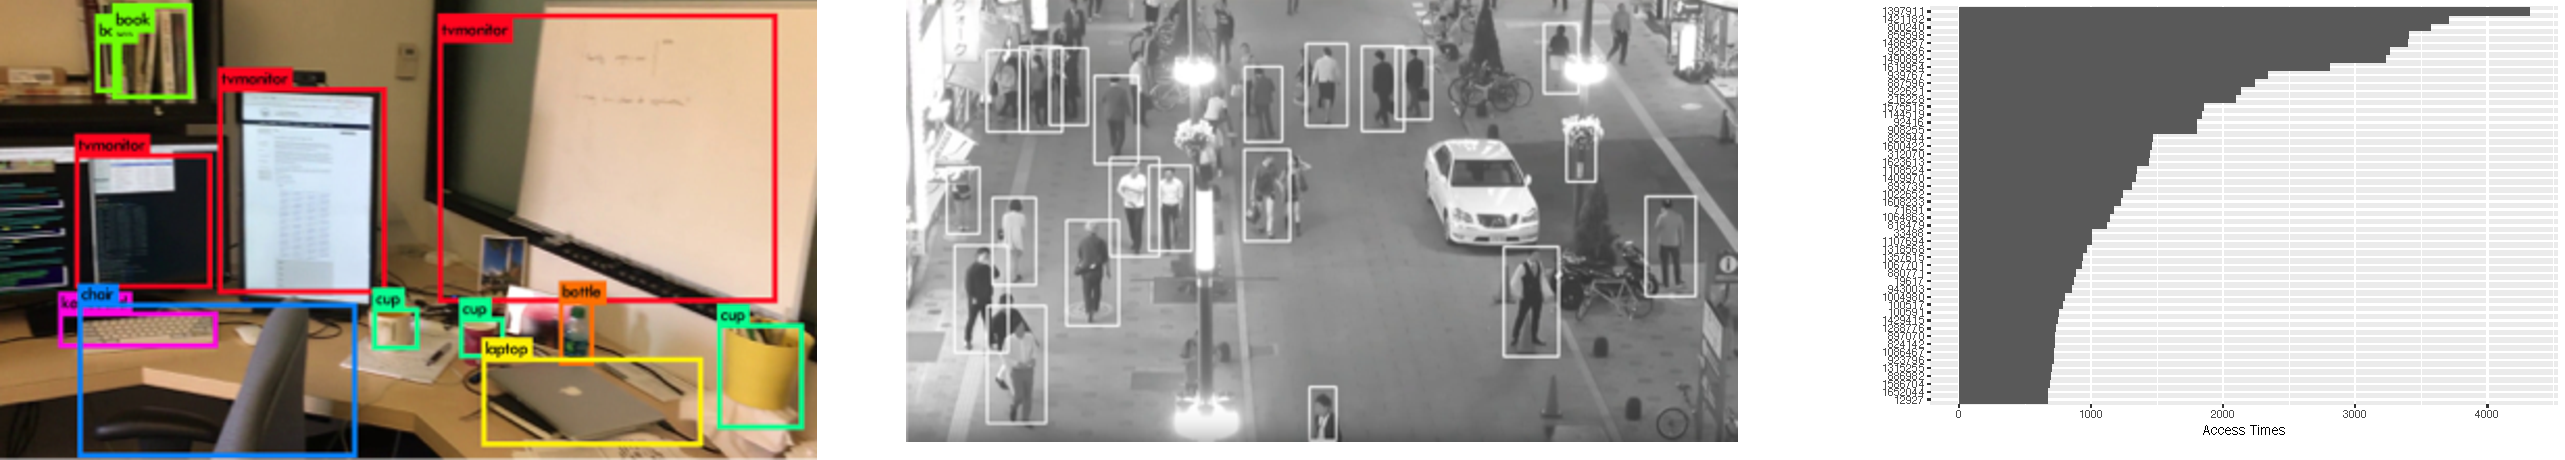
\includegraphics[width=\linewidth]{figures/apps.pdf}
\end{frame}

\begin{frame}{Top-K}
  \centering
  \begin{figure}
    \centering
    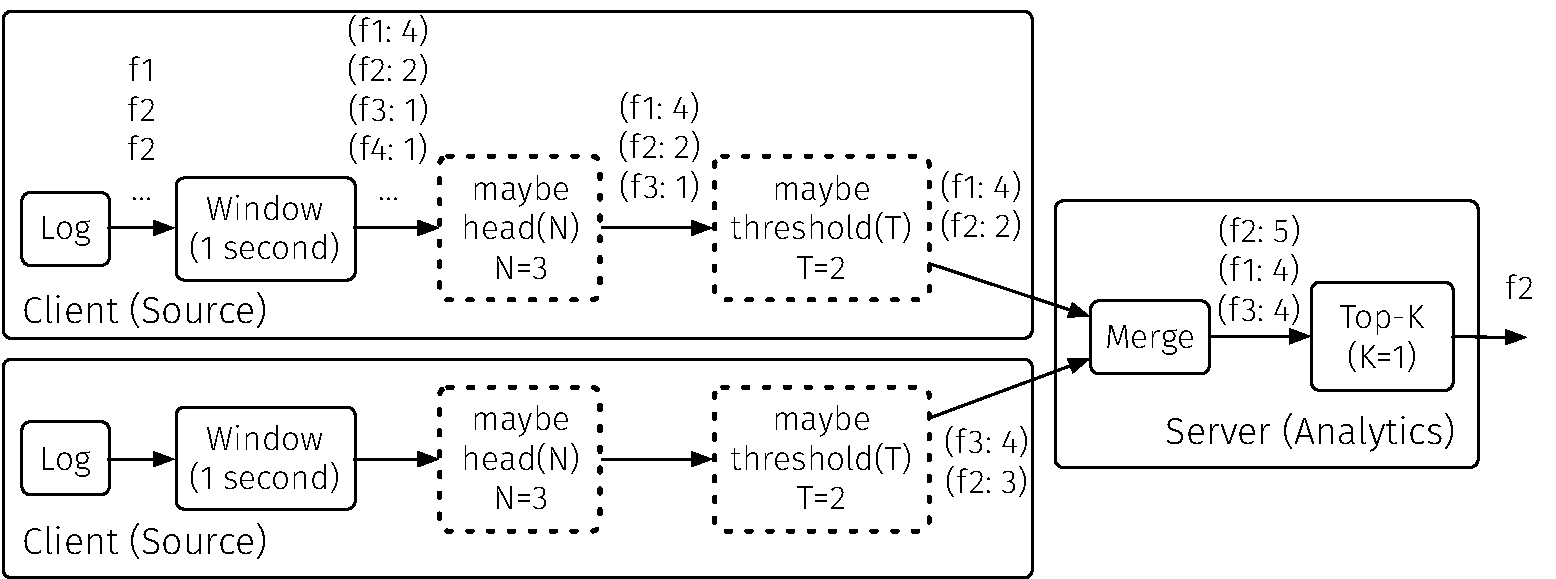
\includegraphics[width=\linewidth]{figures/topk.pdf}
    \caption{A distributed Top-K application with two degradation operations:
      \texttt{head} and \texttt{threshold}. In this example, \texttt{f2}, which
      is not in Top-1 for either client, becomes the global Top-1 after the
      merge. It would have been purged if the clients use threshold T=3,
      demonstrating degradation that reduces data sizes affects fidelity.}
    \label{fig:topk}
    \vspace{-0.5em}
  \end{figure}
\end{frame}

%%% Local Variables:
%%% mode: latex
%%% TeX-master: "../talk"
%%% TeX-engine: xetex
%%% End:

\begin{frame}{Evaluation: Generated Profiles}
  \begin{figure}
    \centering
    \begin{subfigure}[t]{0.48\textwidth}
      \centering
      \caption{Augmented Reality (AR)}
      \label{fig:ar-profile}
      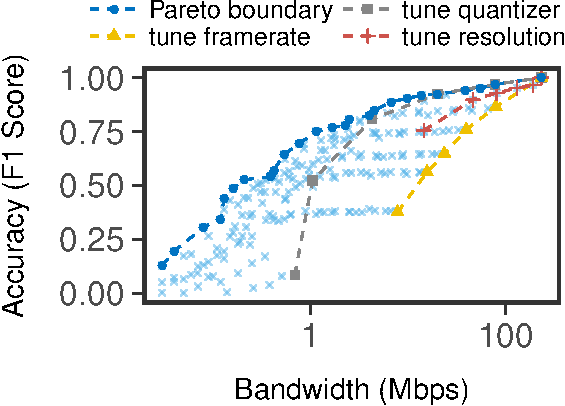
\includegraphics[width=\textwidth]{figures/profile-darknet.pdf}
    \end{subfigure}
    \hfill
    \begin{subfigure}[t]{0.48\textwidth}
      \centering
      \caption{Pedestrian Detection (PD)}
      \label{fig:pd-profile}
      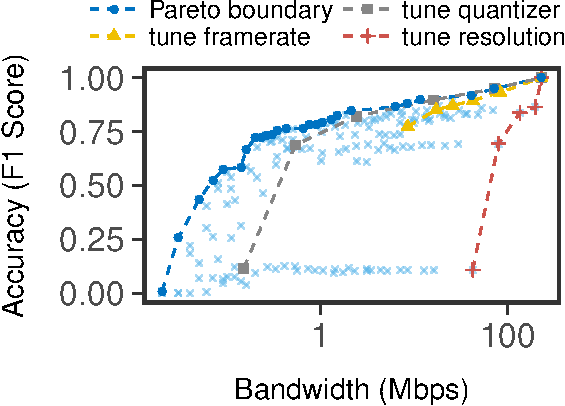
\includegraphics[width=\textwidth]{figures/profile-mot.pdf}
    \end{subfigure}
  \end{figure}

  \begin{itemize}
    \footnotesize
    \visible<2->{
    \item Optimal strategy is achieved with multiple dimensions; tuning one
      dimension leads to suboptimal performance.
    }
    \visible<3->{
    \item For the same application, different dimensions have different impact.
    }
    \visible<4->{\item For different applications, the same dimension has different
      impact.
    }
  \end{itemize}
\end{frame}

\begin{frame}{Evaluation: Generated Profiles (Top-K)}
  \begin{columns}
    \begin{column}{0.45\textwidth}
      \begin{figure}
        \centering
        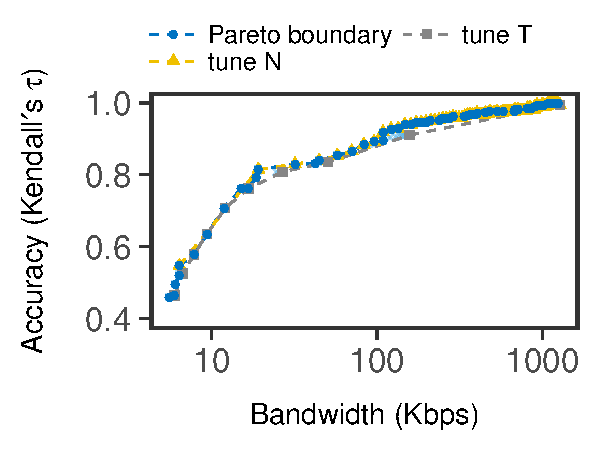
\includegraphics[width=\textwidth]{figures/profile-topk.pdf}
      \end{figure}
    \end{column}
    \begin{column}{0.55\textwidth}
      \begin{itemize}
        \visible<2->{
        \item The effect of each dimension is not significantly different.
        }
        \visible<3->{
        \item The profile offers quantified effects of degradation.
        }
      \end{itemize}
    \end{column}
  \end{columns}
\end{frame}

\begin{frame}{Evaluation: Runtime Experiment Baselines}
  \vspace{1em}
  \only<1-4>{
  \begin{table}
    \footnotesize
    \centering
    \begin{tabular}{ c m{0.6\linewidth} }
      \toprule
      \textbf{Baseline} & \textbf{Description} \\
      \midrule
      Streaming over TCP & A non-adaptive approach \\
      \midrule
      Streaming over UDP & A non-adaptive approach, represents RTP/UDP/RTSP
                           video streaming \\
      \midrule
      \visible<2->{
      \specialcell{JetStream\\\cite{rabkin2014aggregation}}
                        & Manual Policy: \textit{``if bandwidth is insufficient, switch to
                          sending images at 75\% fidelity, then 50\% if there still isn't enough
                          bandwidth. Beyond that point, reduce the frame rate, but keep the image
                          fidelity.''} \\
      \midrule
      }
      \visible<3->{
      JetStream++ & Uses adaptation policy generated by AWStream. JetStream
                    runtime does not probe (hence may oscillate between policies). \\
      \midrule
      }
      \visible<4->{
      \specialcell{HLS\\\cite{pantos2016http}}
                        & HTTP Live Streaming represents popular adaptive video
                          streaming techniques; used for Periscope video stream~\cite{wang2016anatomy}. \\
      \bottomrule
      }
    \end{tabular}
  \end{table}
  }

  \only<5->{
    \begin{figure}
      \centering
      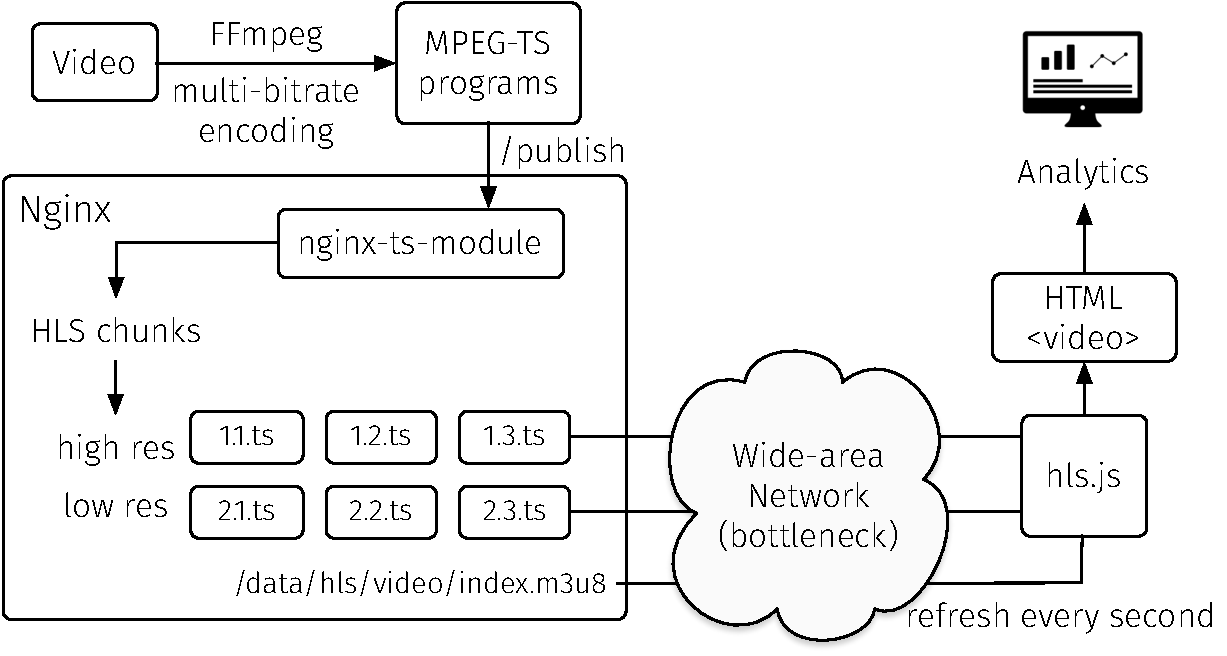
\includegraphics[width=0.8\textwidth]{figures/hls.pdf}
      \caption{HTTP Live Streaming (HLS) architecture: designed for live video
        viewing and relying on buffering at the viewing side.}
    \end{figure}
  }
\end{frame}

\begin{frame}{Evaluation: Runtime Performance}
  \only<1-5>{
    \begin{figure}
      \centering
      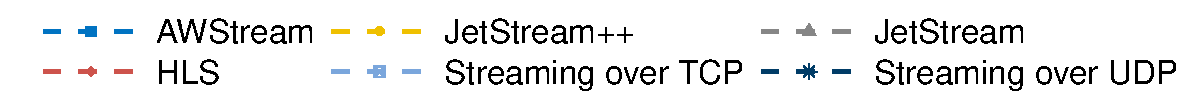
\includegraphics[width=0.8\textwidth]{figures/runtime-timeseries-legend.pdf}
    \end{figure}
    \vspace{-1em}
  }
  \only<1>{
    \begin{figure}
      \centering
      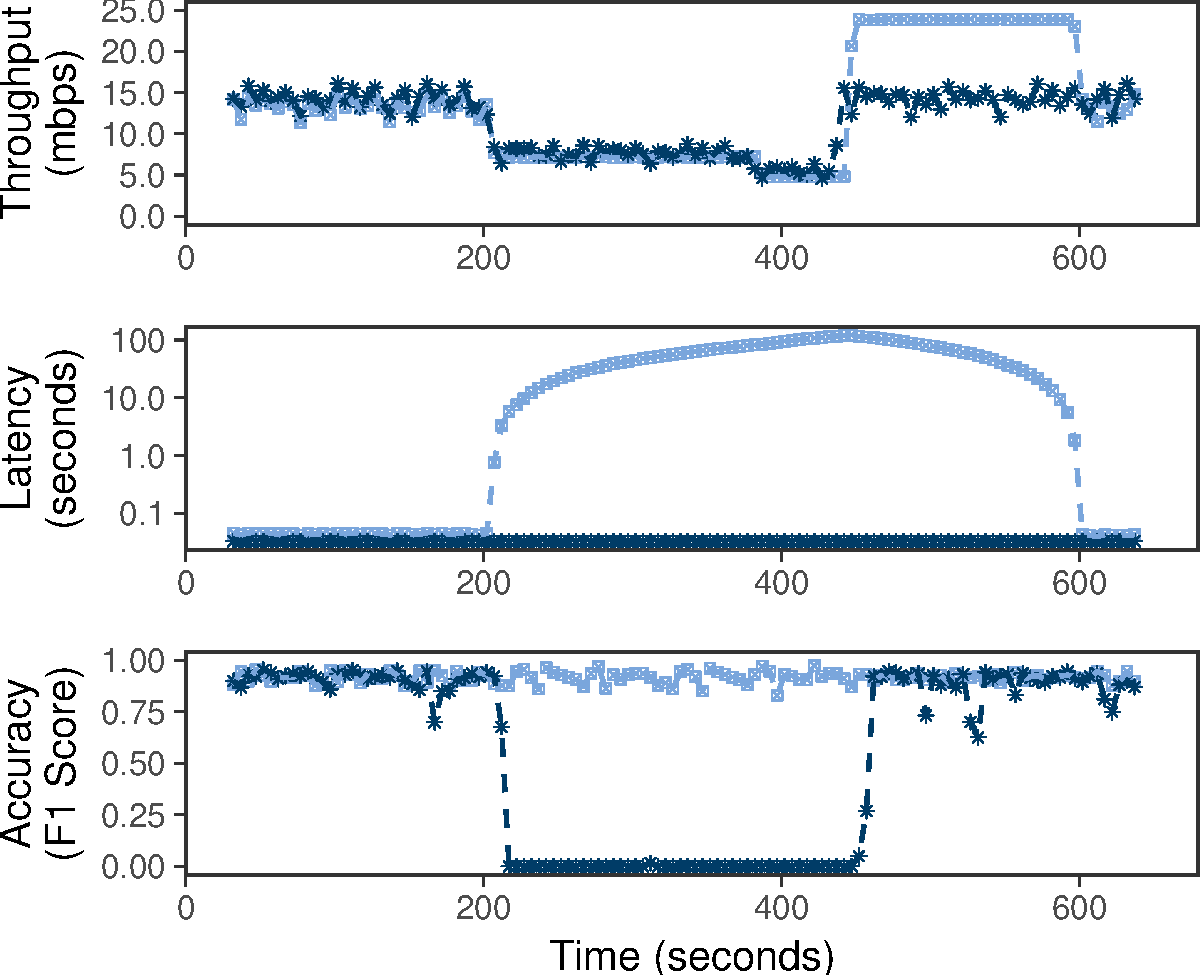
\includegraphics[width=0.8\textwidth]{figures/runtime-timeseries-1.pdf}
    \end{figure}
  }
  \only<2>{
    \begin{figure}
      \centering
      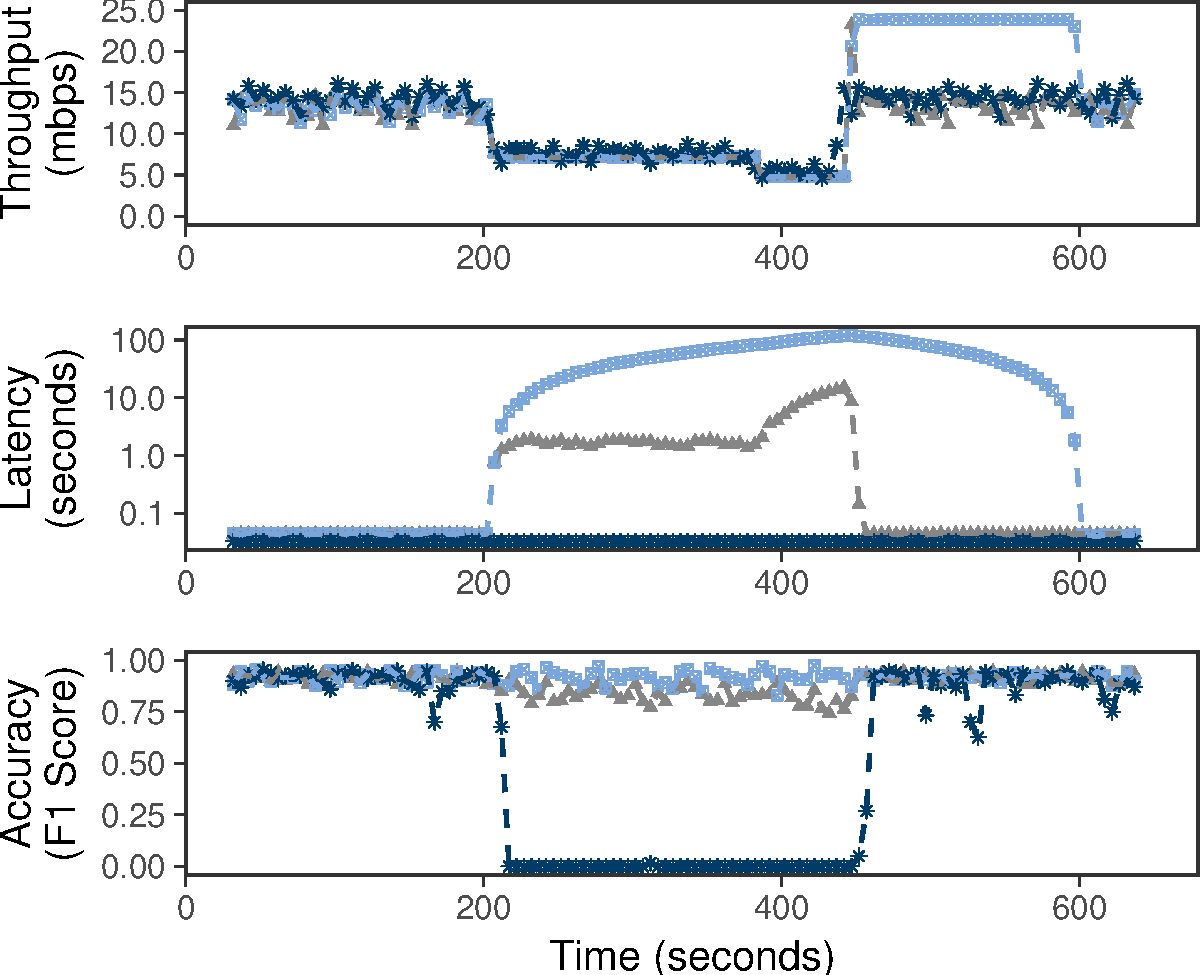
\includegraphics[width=0.8\textwidth]{figures/runtime-timeseries-2.pdf}
    \end{figure}
  }
  \only<3>{
    \begin{figure}
      \centering
      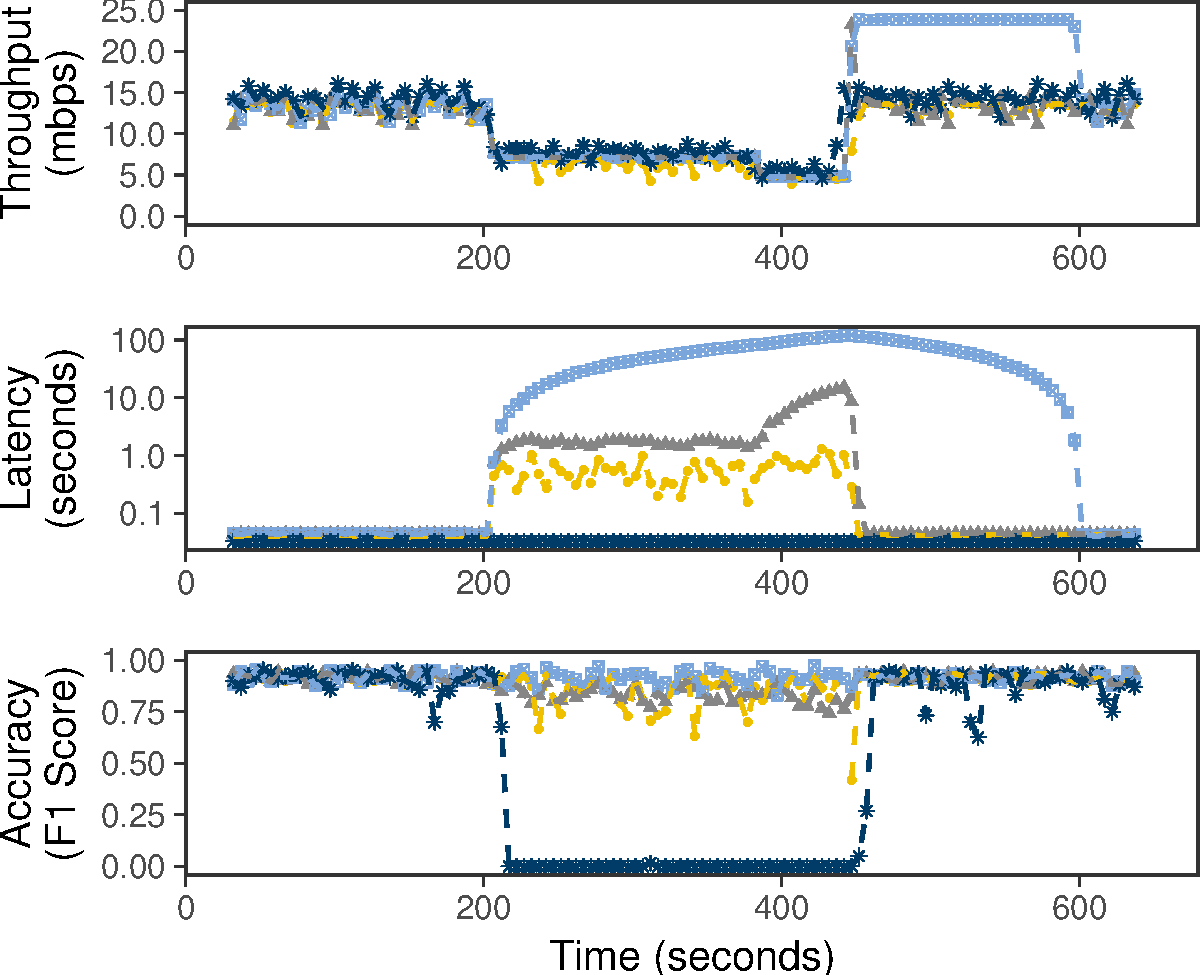
\includegraphics[width=0.8\textwidth]{figures/runtime-timeseries-3.pdf}
    \end{figure}
  }
  \only<4>{
    \begin{figure}
      \centering
      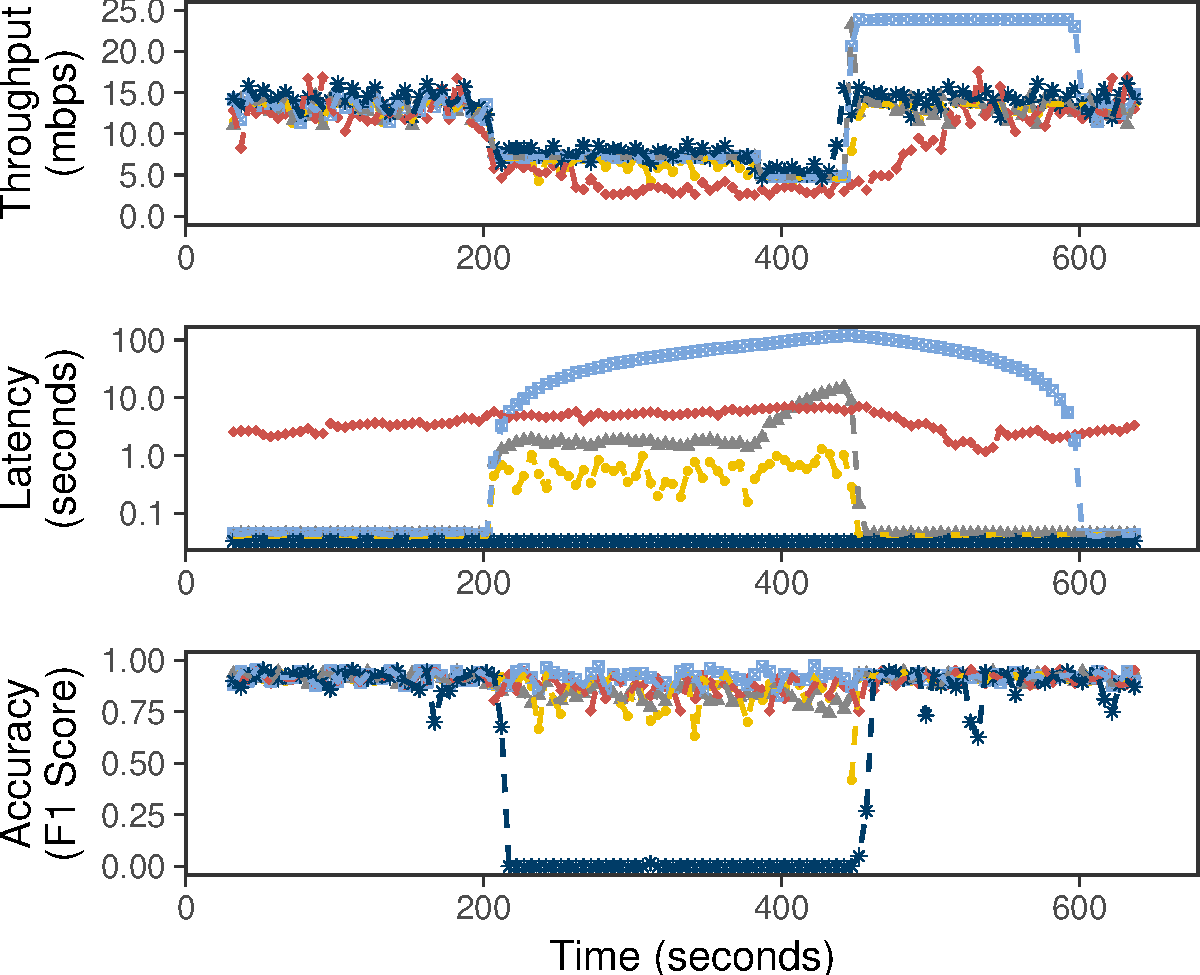
\includegraphics[width=0.8\textwidth]{figures/runtime-timeseries-4.pdf}
    \end{figure}
  }
  \only<5>{
    \begin{figure}
      \centering
      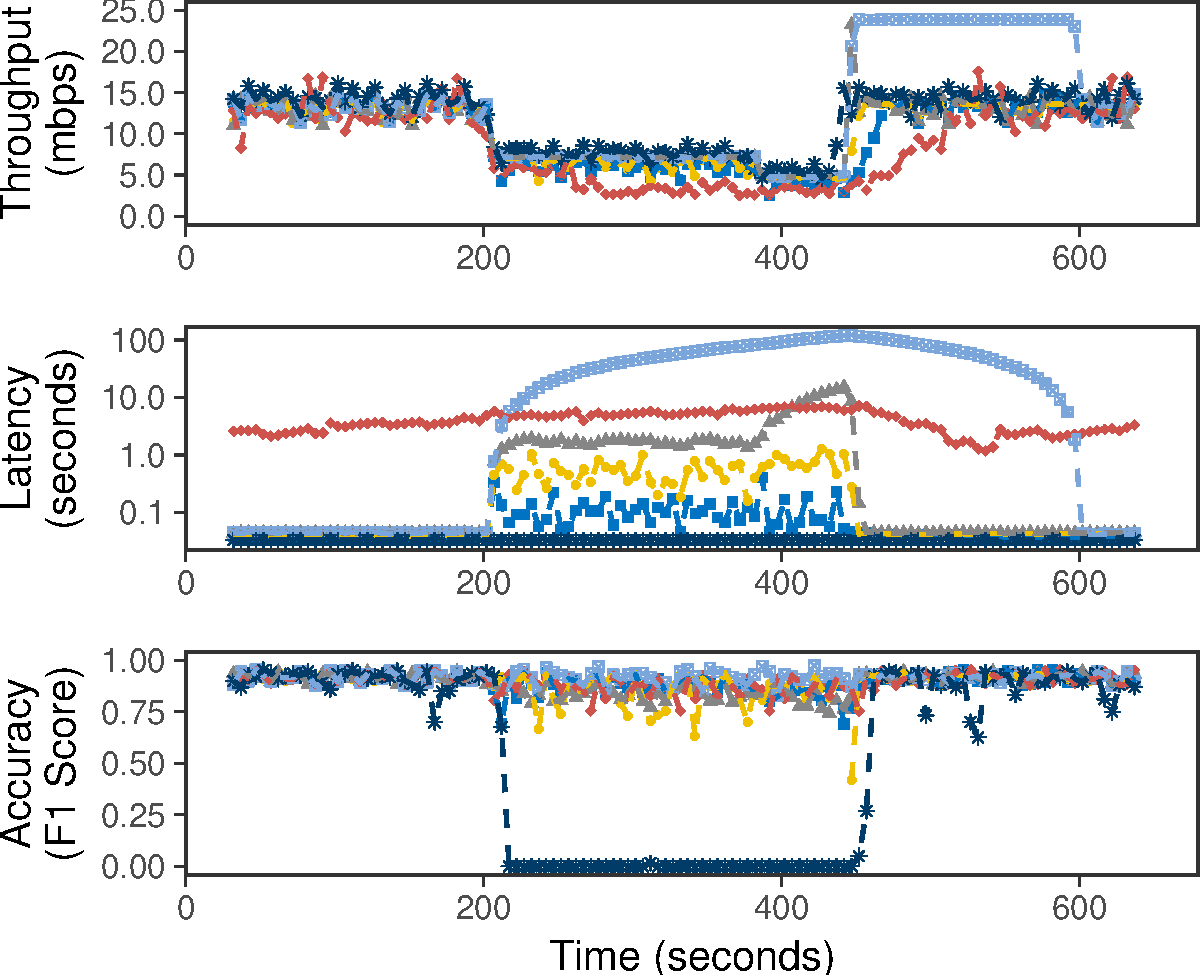
\includegraphics[width=0.8\textwidth]{figures/runtime-timeseries-5.pdf}
    \end{figure}
  }

  \only<6->{
    \begin{figure}
      \centering
      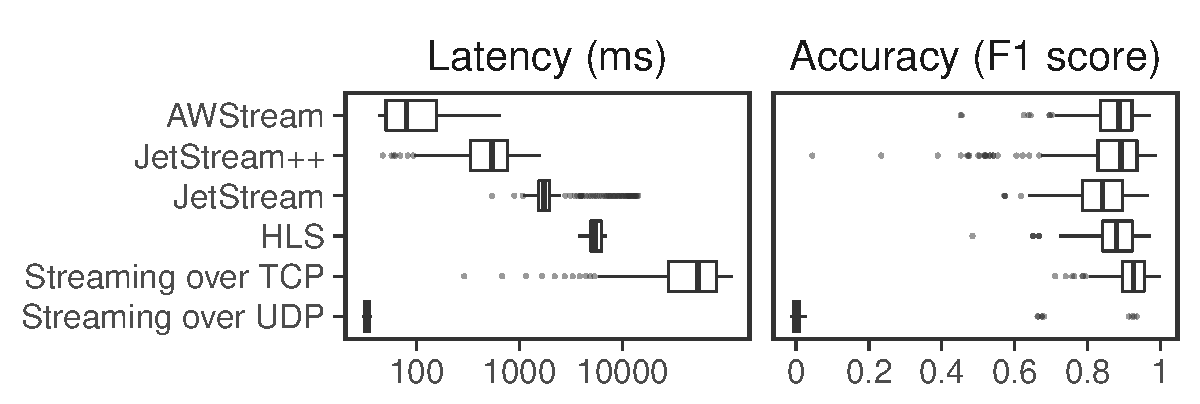
\includegraphics[width=0.8\textwidth]{figures/runtime-boxplot.pdf} \\
      \vspace{1em}
      \visible<7>{
        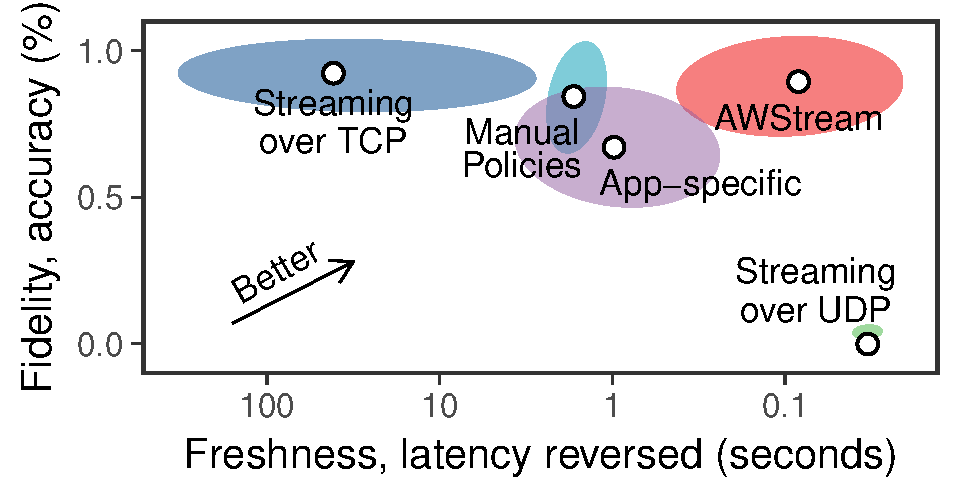
\includegraphics[width=0.6\columnwidth]{figures/fidelity-freshness-full.pdf}
      }
    \end{figure}
  }
\end{frame}

%%% Local Variables:
%%% mode: latex
%%% TeX-master: "../talk"
%%% TeX-engine: xetex
%%% End:



\begin{frame}{All Profiles}
  \begin{figure}
    \includegraphics[width=0.9\linewidth]{figures/runtime_darknet-timeseries.pdf}
  \end{figure}
\end{frame}

%%% Local Variables:
%%% mode: latex
%%% TeX-master: "talk"
%%% TeX-engine: xetex
%%% End:
